%!TEX root = main.tex

\newpage
\section{Реализация ОА}

Для реализации цифрового автомата использовалась САПР <<Альтера>> Max+plus II.

\subsection{Реализация ОА${}_1$}

\begin{figure}[H]
	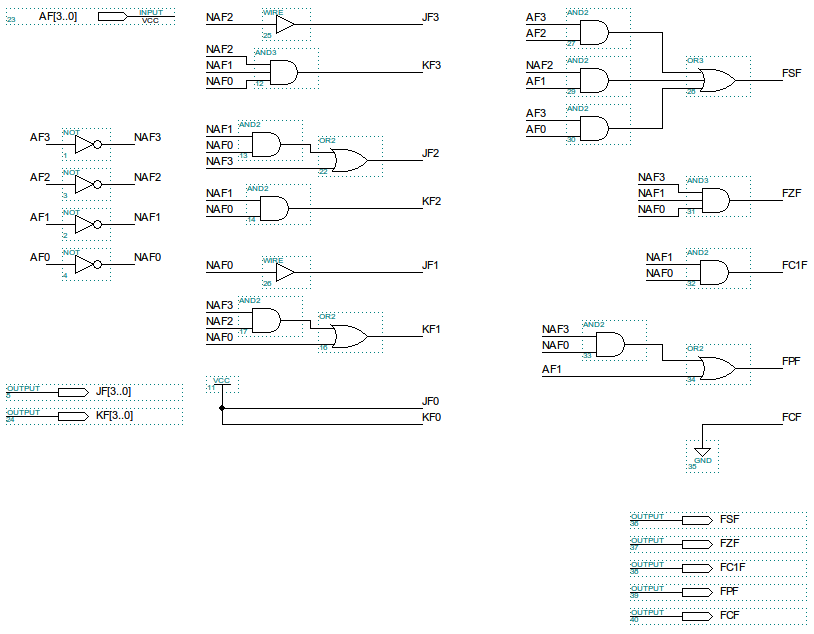
\includegraphics[scale=0.6]{images/altera/oa10_logic.png}
	\caption{Схема ОА$^{(0)}_{1}$}
	\label{figure:oa10log}
\end{figure}

\begin{figure}[H]
	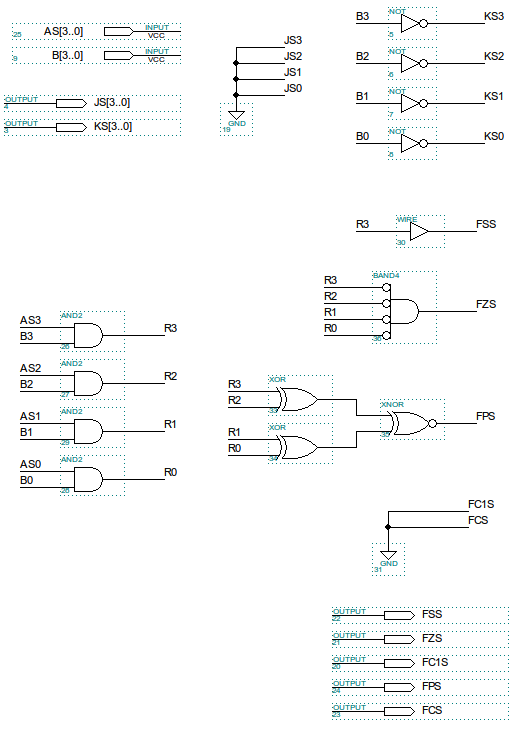
\includegraphics[scale=0.6]{images/altera/oa11_logic.png}
	\caption{Схема ОА$^{(1)}_{1}$}
	\label{figure:oa11log}
\end{figure}

\begin{figure}[H]
	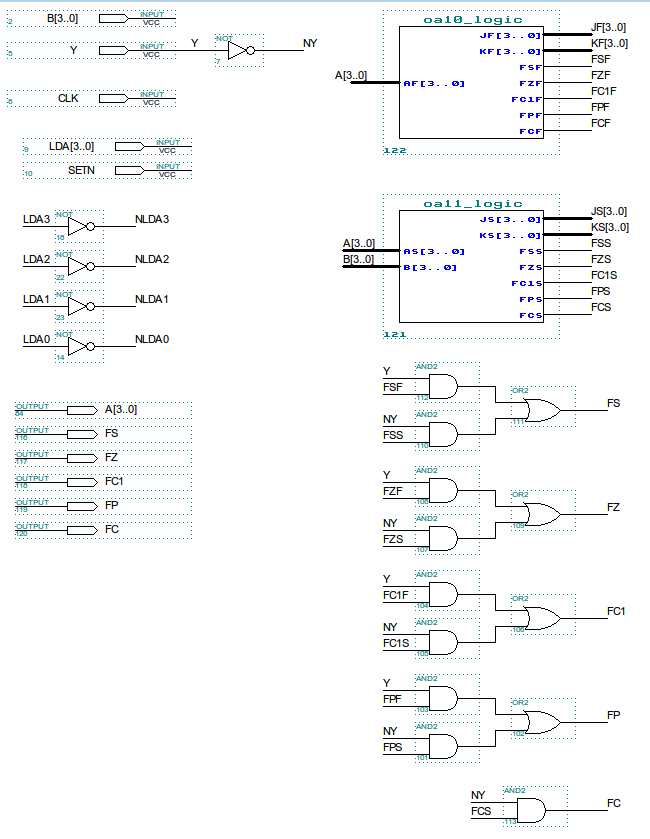
\includegraphics[scale=0.6]{images/altera/oa1_1.png}
	\caption{Cхема ОА$_{1}$ (начало)}
	\label{figure:oa1-1log}
\end{figure}

\begin{figure}[H]
	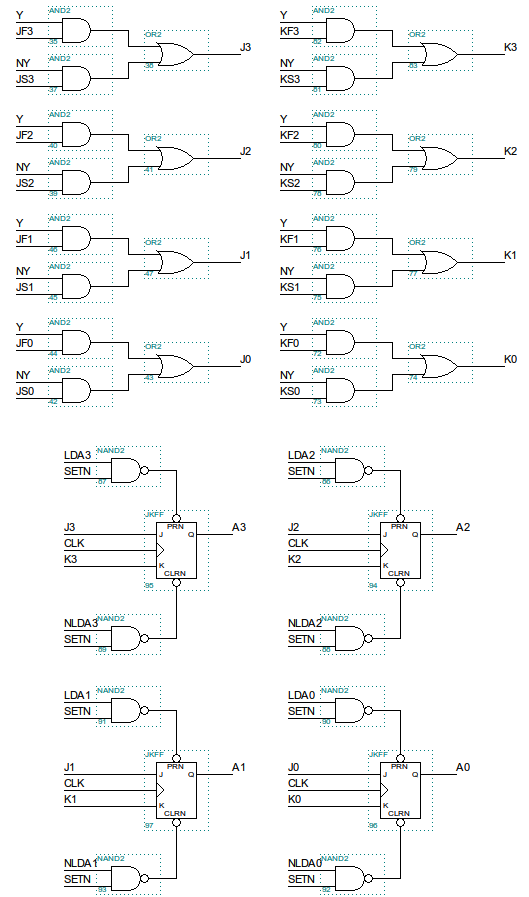
\includegraphics[scale=0.6]{images/altera/oa1_2.png}
	\caption{Cхема ОА$_{1}$ (окончание)}
	\label{figure:oa1-2log}
\end{figure}


\clearpage
\subsection{Реализация ОА${}_2$}

\begin{figure}[H]
	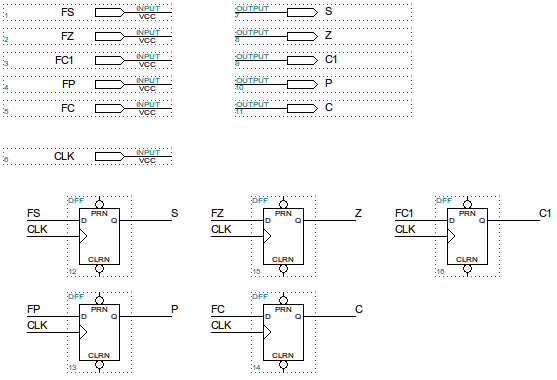
\includegraphics[scale=0.6]{images/altera/oa2.png}
	\caption{Cхема ОА$_{2}$}
	\label{figure:oa2log}
\end{figure}

\subsection{Реализация ОА}

\begin{figure}[H]
	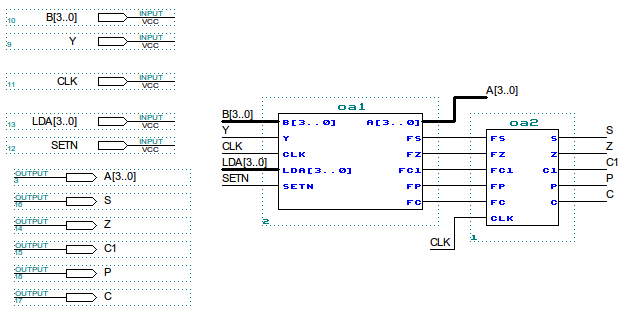
\includegraphics[scale=0.6]{images/altera/oa.png}
	\caption{Cхема ОА}
	\label{figure:oalog}
\end{figure}

\newpage
\section{Моделирование ОА}

\subsection{Методика моделирования}

Процесс моделирования данного автомата был разделен на 3 этапа:
\begin{itemize}
	\item Моделирование ОА$_1$. Целью моделирования ОА1 является проверка правильности выполнении операций, проверка формирования значений логических функций признаков $f_S$, $f_Z$, $f_{C'}$, $f_P$, $f_C$. 
	\item Моделирование ОА$_2$. На данном этапе осуществляется проверка правильности записи значений признаков $S$, $Z$, $C'$, $P$, $C$.
	\item Моделирование ОА. На данном этапе осуществлялась проверка правильности взаимодействия автоматов ОА$_1$ и ОА$_2$. 
\end{itemize}

\subsection{Выполнение арифметической операции}








\subsection{Выполнение логической операции}